%% A simple branched neurons.
\documentclass[tikz]{standalone}
\usetikzlibrary{arrows,decorations,calc}
\usetikzlibrary{decorations.pathmorphing}
\usetikzlibrary{intersections}

\begin{document}

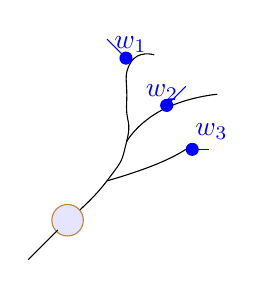
\begin{tikzpicture}[scale=1
        , every node/.style={}
    ]

    \node[] (soma) at (0,0) {}; 
    \node[] (A) at (0.5,0.5) {};
    \node[] (B) at (0.75,1.0) {};
    \node[] (synA) at (0.8, 2.0) {};
    \node[] (synB) at (1.2,1.4) {};
    \node[] (synC) at (1.5,0.9) {};

    \draw plot [smooth, tension=1] coordinates {
        (0,0) (A) (B) (0.75,1.5) (synA) (1.1,2.1)
    };
    \draw plot [smooth, tension=1] coordinates {
        (B) (synB) (1.9,1.6)
    };
    \draw plot [smooth, tension=1] coordinates {
        (A) (1.1,0.7) (synC)
    };

    %% soma is round 
    \fill[blue!10
        , draw=brown
        %, decorate
        %, decoration={random steps, segment length=0.1, amplitude=0.1}
        , name path = somap
    ] (soma) ellipse (0.2 and 0.2);

    % output is small axon.
    \draw[-] (soma) -- ++(-0.5,-0.5);

    % lets draw synapses now.
    \draw[*-, blue] (synA.center)  node[above] {$w_1$} -- ++(-0.3,0.3);
    \draw[*-, blue] (synB.center)  node[above] {$w_2$} -- ++(.3,0.3);
    \draw[*-, blue] (synC.center)  node[above right] {$w_3$} -- ++(.3,0);
\end{tikzpicture} %
\end{document}

